\documentclass{tufte-book}

\hypersetup{colorlinks}% uncomment this line if you prefer colored hyperlinks (e.g., for onscreen viewing)

%%
% Book metadata
\title{Hypercompression}
\author{Charles Holbrow}
%\publisher{Publisher of This Book}

%%
% If they're installed, use Bergamo and Chantilly from www.fontsite.com.
% They're clones of Bembo and Gill Sans, respectively.
%\IfFileExists{bergamo.sty}{\usepackage[osf]{bergamo}}{}% Bembo
%\IfFileExists{chantill.sty}{\usepackage{chantill}}{}% Gill Sans

%\usepackage{microtype}

%%
% Symbol for Euro Currency
\usepackage[official]{eurosym}

%%
% For nicely typeset tabular material
\usepackage{booktabs}

%%
% For graphics / images
\usepackage{graphicx}
\setkeys{Gin}{width=\linewidth,totalheight=\textheight,keepaspectratio}
\graphicspath{{graphics/}}

% The fancyvrb package lets us customize the formatting of verbatim
% environments.  We use a slightly smaller font.
\usepackage{fancyvrb}
\fvset{fontsize=\normalsize}

%%
% Prints a trailing space in a smart way.
\usepackage{xspace}

% Inserts a blank page
\newcommand{\blankpage}{\newpage\hbox{}\thispagestyle{empty}\newpage}

\usepackage{units}
% Control the formatting of lists
\usepackage{enumitem}

% Typesets the font size, leading, and measure in the form of 10/12x26 pc.
\newcommand{\measure}[3]{#1/#2$\times$\unit[#3]{pc}}

% Macros for typesetting the documentation
\newcommand{\hlred}[1]{\textcolor{Maroon}{#1}}% prints in red
\newcommand{\hangleft}[1]{\makebox[0pt][r]{#1}}
\newcommand{\hairsp}{\hspace{1pt}}% hair space
\newcommand{\hquad}{\hskip0.5em\relax}% half quad space
\newcommand{\TODO}[1]{\textcolor{red}{\bf TODO:#1}\xspace}
\newcommand{\ie}{\textit{i.\hairsp{}e.}\xspace}
\newcommand{\eg}{\textit{e.\hairsp{}g.}\xspace}
\newcommand{\na}{\quad--}% used in tables for N/A cells

% Number parts and chapters
\setcounter{secnumdepth}{0}

% Title of my thesis project
\newcommand{\thesis}{Hypercompression\xspace}

\begin{document}

% Front matter
\frontmatter

% Full title page
\maketitle

% Contents
\tableofcontents

% Start the main matter (normal chapters)
\mainmatter

\chapter*{Abstract}
\label{ch:abstract}

\marginnote{\TODO{ Abstract is copy/pasted from another section, and
    should probably be re-written from scratch}} While compression of
mono and stereo audio is well documented and
understood,\cite{Giannoulis2012, Blesser1969} surround sound
compression is relatively less explored.  \thesis expands on
traditional audio compression model by adding spatial control. This
design introduces two additional high level spatial parameters:
\textbf{link angle} and \textbf{spread}. These parameters extend the
domain of the traditional compressor to include surround sound spatial
manipulation in addition to dynamics processing, and unlock new
creative possibilities for surround sound designers.


% Introduction
\cleardoublepage
\chapter{Introduction}
\label{ch:introduction}

In the 6th Century BC, Pythagoras notices that that blacksmith's
hammers of different sizes created different pitches when struck on an
anvil.\cite{Weiss2007} He identified that some ratios of weights
created dissonant sounds, while some created consonant sounds.
Pythagoras is the earliest known example drawing the connection
between music and mathematics. Today, we describe musical pitches, as
integers within a given tuning system. We describe the tuning system
with a mathematical formula that relates frequency to pitch. Musical
time, rhythm and meter are commonly described numerically. Musical
Transposition and inversion mirror mathematical functions, and borrow
their names directly from mathematics. As computers, amplifiers and
electronics become our primary tools for creating manipulating, and
performing music, mathematics and music have become more
interconnected. Nearly every modern musical recording, broadcast, and
stream is the sumation of many digital recordings that have been
individually discretized, sampled mathematically encoded, and
digitally processed numerous times before ever reaching our ears. We
might be tempted to describe music as applied mathematics, but doing
so betrays a fundamental quality of music: Musical beauty does not
correspone mathematical beauty. A vocalist does not abruptly change a
pitch, but gently and carefuly lands on a pitch. A jazz musician might
play slightly \emph{behind the beat}. A classical performer knows how
to hold a fermata \emph{just long enough}. These intentional human
artifacts artifacts are characterised more by a \emph{feeling} than by
a formula.

The computer's inability to understand feeling, opened possibilities
for new genres of music like EDM\sidenote{EDM (Electronic Dance Music)
  features formulaic grooves perfectly locked to a grid, and often
  aggressive use of digital pitch correction exagerating a robotic
  quality.}, Black MIDI\sidenote{Black MIDI is a musical genre that
  uses low fidelity audio samplers with a large number of midi
  notes. A single 3 minute Black MIDI track is likely to have over
  100,000 MIDI notes. The name refers to the solid black appearance of
  the piano score.}, and Demoscene Music\sidenote{Demoscene music
  celebrates the computationally efficient generation of complex
  digital music.}. These styles of music feature (rather than fix) the
unfeeling nature of computers. If we want computer to produce truely
expressive music we must try to capture percieved feelings
formulaically, and instruct compters to reproduce them.


\section{Hypercompression}
\label{sec:hypercompression-intro}
We usually think of compression in terms of \emph{reduction}: We use
data compression to reduce bit-rates and file sizes, audio compression
to reduce dynamic range. Record labels even use compression as a
weapon in the \emph{loudness war}\cite{Deruty2014a}, resulting in some
of today's music recordings utilizing no more dynamic range than a
1909 Edison cylinder.\cite{Katz2007} A deaper study of compression
reveals more subtle and artistic applications. A skilled audio
engineer applies compression to audio with the intention to improve
intelligibility, augment articulation, smooth a performance, shape
transients, extract ambience, de-ess vocals, balance multiple signals,
or even add distortion.\cite{Case2007} At its best, the compressor is
a tool for \emph{temporal shaping} first, and not a tool for \emph{dynamic
  reduction} second.

\thesis expands the traditional model of a compressor to include
\emph{spatial shaping}. While unconventional, spatial processing is a
very natural fit for the compression paradigm. We can think of sound
as a medium that exists in time just as easily as we can think of
sound as soemthing that exists in space.\sidenote{Converting
  measurement of sound from the cycles per second (in the temporal
  domain) to wavelength (in the spatial domain) is common objective in
  acoustics and audio engineering practices. See \textit{The Sound
    Reinforcement Handbook} by G. Davis for examples.} The
Hypercompressor described in detail in \autoref{ch:hypercompressor}.

\paragraph{Performance}
\TODO{Comments about live performance}

\section{Context}
\label{sec:context}

\newthought{The Phillips Pavilion} stands out as an inspiration, a
reference, and a guide for projects that successfully disregard the
conventional disciplinary approach to the creative design process. The
pavilion was a commissioned by Phillips Corporation for the Brussels
World's Fair in 1958.\cite{Zvonar1999} When the architectural offices of
Le Corbusier received the commission, Le Corbusier replied, saying:
``I will not make a pavilion for you but an Electronic Poem and a
vessel containing the poem; light, color image, rhythm and sound
joined together in an organic synthesis.''\cite{Lopez2011} Indeed,
the pavilion embodied Le Corbusier's description, and the resulting
Gesamtkunstwerk included:\cite{Lombardo2009}
\begin{enumerate}
\item A concrete pavilion, designed by architect and composer Iannis
  Xenakis
\item \textit{Interlude Sonoire} (later renamed \textit{Concret PH}), a
  tape music composition by Iannis Xenakis, approximately 2 minutes
  long, played while the audience transitioned
\item A three channel, 8 minute tape music composition, by French-born
  composer Edgard Var\`{e}se
\item A system for spatialized audio across at least 350 loudspeakers
  distributed throughout the pavilion
\item An assortment of visual effects, designed by Le Corbusier in
  collaboration with Philips art director Louis Kalff
\item Video consisting mostly of black and white still images,
  projected on two walls inside the pavilion
\item A system for synchronizing playback of audio and video playback,
  with light effects and audio spatialization throughout the
  experience
\end{enumerate} 

It is a little surprising that Le Corbusier chose Iannis Xenakis, a
young engineer with no formal architectural training to design the
pavilion building, and compose a part of the music. While the
relationship between Le Corbusier and Xenakis would deteriorate as a
result of their work on Philips Pavilion, there was probably no one
better equipped than Xenakis to merge the fields of music, mathematics
and architecture. To understand Xenakis' impact on the project, we
have to review the influences and experiences that led him to Paris
and to Le Corbusier's architecture firm in 1947.

\subsection{The Influence of Iannis Xenakis}
\label{sec:influence-xenakis}

Xenakis was born in Romania in 1922, and moved to Greece in 1932. He
left school at the age of 16, and spent his time reading about
astronomy, archeology, ancient literature, and
mathematics.\cite[]{Hoffmann2015} He was admitted to the
Polytechnic Institute in Athens in 1940, where he studied music,
counterpoint, and engineering. While attending the Polytechnic
Institute, he fought with the resistance against the Nazi Invasion in
Greece. He was jailed and tortured multiple times for his involvement
with the resistance, and eventually sentenced to death for terrorism,
but managed to escape.\cite[]{Simms2014} In 1946 he received his
degree in engineering from the Polytechnic Institute, and left Greece
the following year, using a forged passport.\cite[]{Prendergast2014}

Xenakis began working for Le Corbusier in 1948, but he continuted to
study and write music. While Xenakis was searching for a music mentor,
he approached Oliver Messiaen\sidenote{Messiaen was a well known
  french composer known for rhythmic complexity, and transcribing
  birdsong into his music.}, and asked if he should study harmony or
counterpoint. Messiaen later described his conversation with
Xenakis:

\begin{quotation}``I think one should study harmony and
  counterpoint. But this was a man so much out of the ordinary that I
  said: No, you are almost 30, you have the good fortune of being
  Greek, of being an architect and having studied special
  mathematics. Take advantage of these things. Do them in your
  music.''\cite{Service2013}
\end{quotation}

Ultimately, Messiaen was rejecting Xenakis as a student, but we can
see how Xenakis did draw from disparate skills in his composition. The
score for his 1945 composition \textit{Metastasis}
(figure~\ref{fig:metastasis}), resembles an architectural blueprint as
much as it does a music score.

\begin{figure*}[h]
  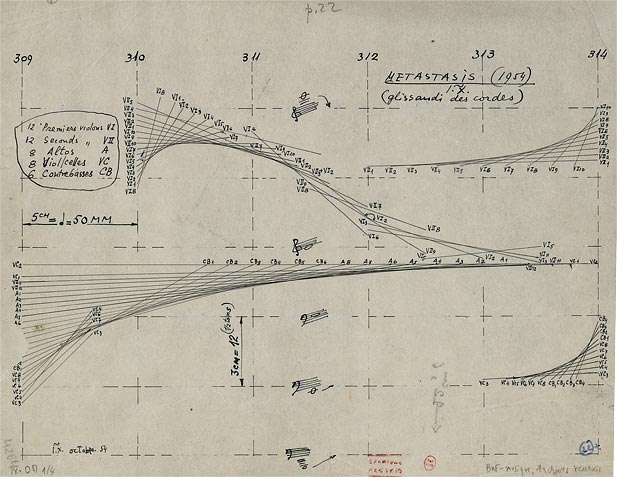
\includegraphics[width=\linewidth]{XenakisMetastasis.jpg}
  \caption{Excerpt from Iannis Xenakis' composition,
    \textit{Metastasis} (1954), measures 309-314. This score was then
    transcribed to sheet music for the orchestral performance.}
  \label{fig:metastasis}
\end{figure*}

In 1956, Le Corbusier was focusing much of his attention on a larger
project; Chandigarh, a city in India on the edge of the Himalayan
plains. When he was approached by Louis Kalff and asked to build a
pavillion for the 1958 World's Fair in Brussels, he immediately
accepted. Kalff wanted the pavilion to showcase the sound and lighting
potential of Philips' technologies. Le Corbusier determined that
the shape of the building should resemble a stomach, with the audience
entering through one entrance, and exiting through another. Thinking
the design of the entire city of Chandigarh would be the masterpiece
of his Architectural career,\cite{Flint2013} he delegated the design
of the pavilion building to Xenakis.\cite{Clarke2012}

\paragraph{Polymath} The architectural evolution of the pavillion from
Le Corbusier's early designs (figure~\ref{fig:le-corbusier-sketch})
through Xenakis' iterations (figure~\ref{fig:xenakis-draw}),
illustrates the impact that Xenakis had on the project. The
\textit{Philips Technical Review}\cite{philips1958} gives a
wonderfully detailed account of Xenakis' process:
\begin{enumerate}
\item Xenakis was aware that parallel walls, or concave spherical
  walls would negatively impact audio perceptibility due to repeated
  or localized acoustic reflections.
\item To acomodate musical purpose of the space he decided to explore
  surfaces with varying curvature...
\item ...leading him to consider ruled
  surfaces\sidenote{\TODO{Explain}} such as the conoid and hyperbolic
  parabaloid.
\end{enumerate}
We see Xenakis utilizing the drafting skills that he learned at the
Polytechnic Instutute and continuted to develop while working with Le
Corbusier. He also understood the mathematical focumation of the ruled
surfaces that make up the structure. These surfaces even look familiar
from the Metastasis score (figure~\ref{fig:metastasis}).

\TODO{The important thing is to understand how Xenakis could not have
synthesized such a progressive and creative structure if he had been
trained in only a single discipline... we see the value of his
interdisciplinary background}

\begin{figure*}[h]
  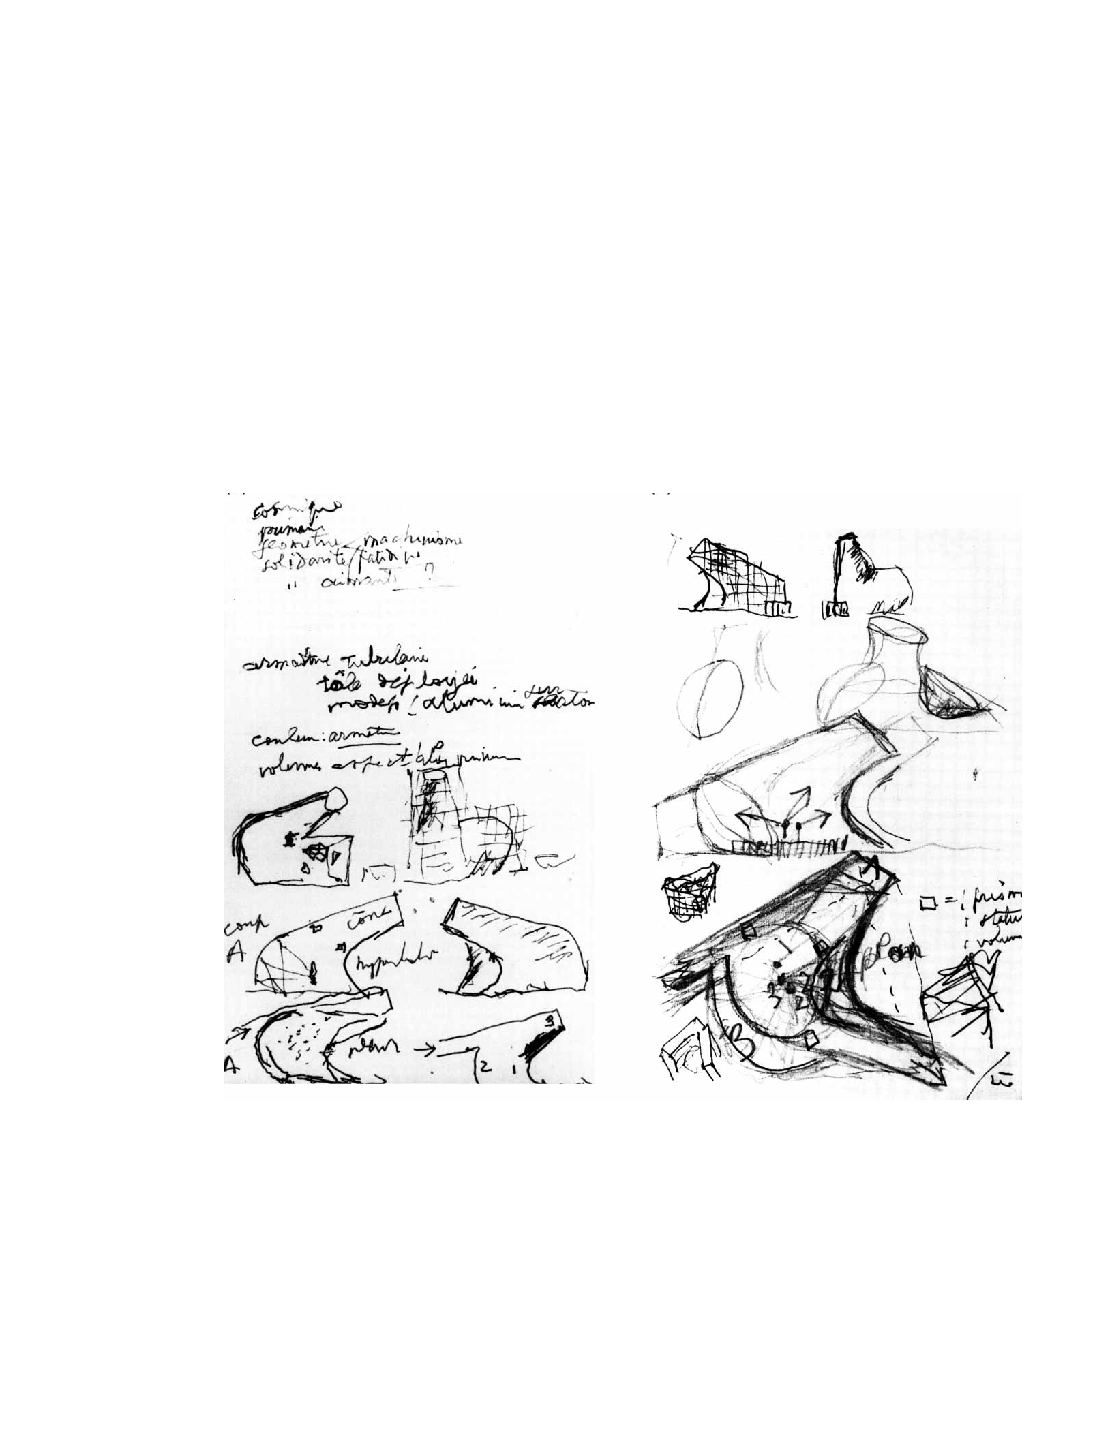
\includegraphics[width=\linewidth]{LeCorbusierDraw.pdf}
  \caption{Le Corbusier's design sketches for the Philips Pavilion,
    September \textendash{} October, 1956 (\textcircled{c} 2012
    Artists Rights Society, New York/ADAGP, Paris/FLC)}
  \label{fig:le-corbusier-sketch}
\end{figure*}

\begin{figure*}[h]
  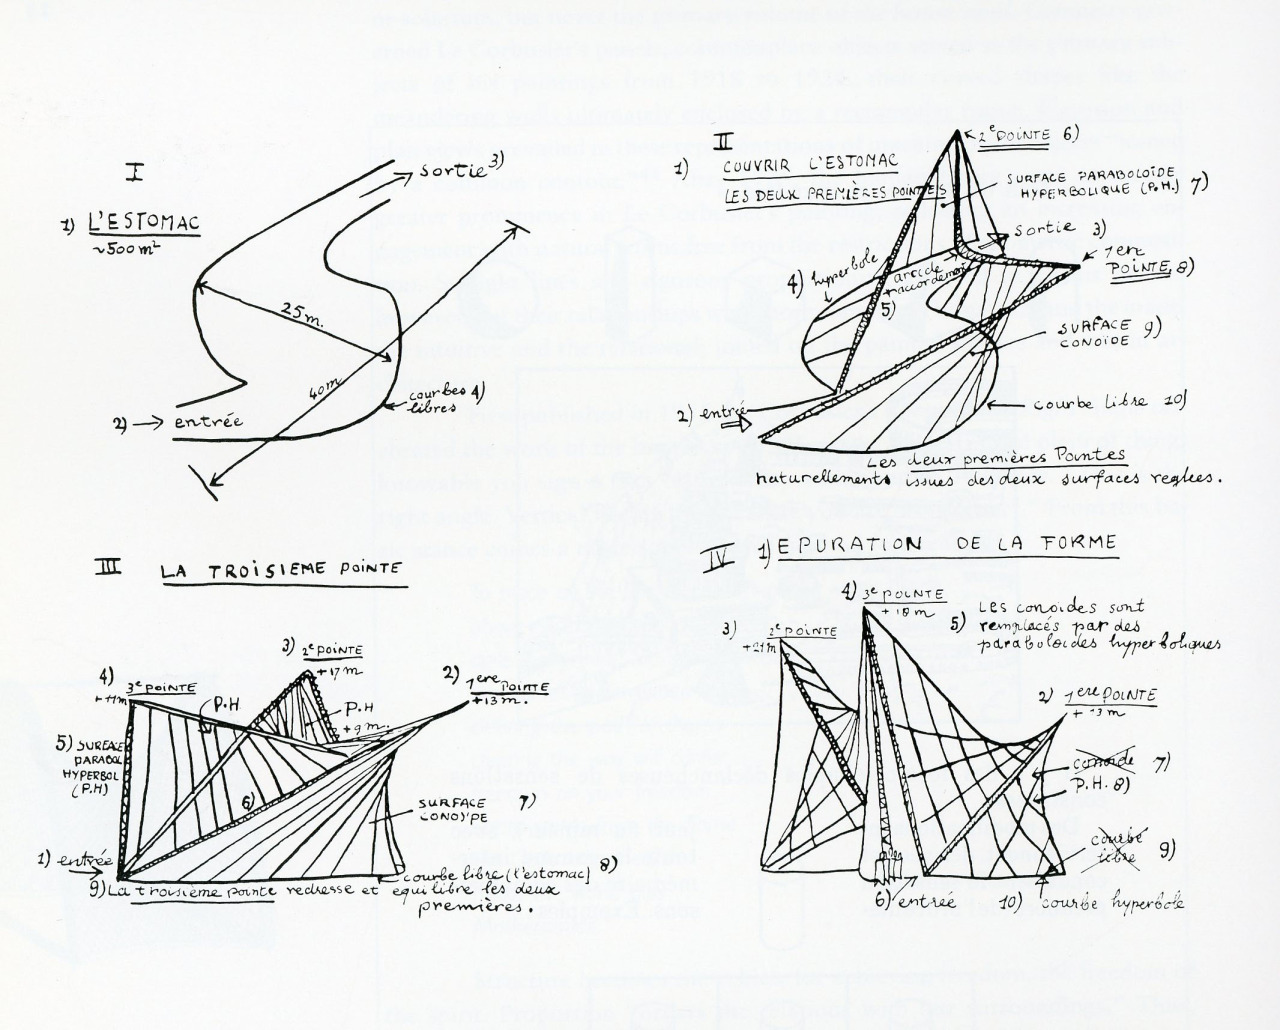
\includegraphics[width=\linewidth]{PhilipsDrawings.jpg}
  \caption{Xenakis' early drawings of the Philips Pavilion as
    documented in the \textit{1958 Philips Technical Review} \TODO{cite}}
  \label{fig:xenakis-draw}
\end{figure*}


\section{Architecture and Music in Space and Time}
\label{sec:introduction-conclusion}

In his 1963 book \textit{Formalized Music}, Xenakis describes how
developments in music theory mimic equivalent developments in
philosophy, mathematics, and the sciences. Polato, for example,
believed that all events transpire as determinted by cause and
effect. While Plato and Aristotle both described causality in their
writing, it was not until the 17th century that controlled experiments
and mathematics coroborated the theory.\sidenote{In 1687, Isaac Newton
  published \textit{Philosophi\ae{} Naturalis Principia Mathematica}
  (\textit{Mathematical Principles of Natural Philosophy}), in which
  he compiled the 3 laws of motion that set the foundation for the
  study of \emph{classical mechanics}.}  Similarly, historical music
follows deterministic progressions, and music theory employs causal
rules to describe counterpoint, tonality, and harmonic movement.

Causality was largely used to describe physical phenomena until the
19th century when statistical theories in physics began to include
probabilistic notions.\sidenote{The Maxwell-Boltzmann distribution,
  which was first derived by James Clerk Maxwell in 1860, describes
  the probability distribution for the speed of a particle within an
  idealized gas. For more see
  \url{http://plato.stanford.edu/entries/statphys-statmech/}} Xenkis
noticed that more contemporary fields like \emph{probability theory}
and \emph{fuzzy logic} generalize and expand on the antecedent
theories of causality.

Xenakis thought that music composition should naturally follow the
progression that physics did, with the theory of music generalizing
and expanding on causal rules that had existed previously. Indeed,
starting in the late 19th century, and early 20th century, composers
like Strauss and Debussy began to bend the existing rules of music
theory, composing music that branched away from the causal and tonal
theories of the time. With the rise of serialism\sidenote{\TODO{Brief
    Serialism Explianation}} and indeterminate
music\sidenote{\TODO{Brief Indeterminate Music explaination}},
composers such as Strauss, Debussy, Stockhausen, Boulez, John Cage,
Aaron Copland, and B\'{e}la Bart\'{o}k began to use probability and
chance in composition, the same way that physicists were using
probability to describe the material world. However, to Xenakis'
mathematical mind, serial music was no less causal than the music it
intended to supersede. He described serial music as embodying
``virtually absolute determinism.''\cite{xenakis1992formalized}
Xenakis saw music theory as a sub-set of mathematics and
algebra. While musicians have a different vocabulary, they also use
mathematical principles to describe and compose music. Because he
understood mathematics as well as music, he was able to identify how
even in serialism and indeterminate music, composers were only utilizing a
small subset of algebraic theory. In his own music, Xenakis wanted to
generalize the and expand the causal framework that musicians and
theorists had been using to compose and understand music. This
paralleled the developments in phyisics and mathematics that helped
him to form his opinions about music theory.  As a nod to
\emph{chance} or \emph{stochos} xenakis coined the term
\emph{stochastic music} to describe this development.

In the Spring of 1976, Xenakis was defending his doctoral thesis at
the University of Paris. A translation of his defense includes this
statement:
\begin{quotation}
  ``The artist-conceptor will have to be knowledgeable and inventive
  in such varied domains as mathematics, logic, physics, chemistry,
  biology, genetics, palentology (for the evolution of forms), the
  human sciences, and history; in short, a sort of
  \emph{universality}, but one based opon, guided by and oriented
  toward forms and architectures.'' \cite{russolo1986art}
\end{quotation}

From Xenakis' drawings we can deduce that he used the same tools,
skills, and philosophy to imagine and concive both music and
space. His approach elevated both forms by blurring the distinction
between the two. Maybe if we had kept using pen and paper to design
buildings and write music, the reality today would be closer to the
ideal that Xenakis imagined. Today, software for creating architecture
and composing music both favor corners to curves, and static pitches
to glissandi. More importantly, the software skills that we use to
design and maniuplate space are not transferable to the composition of
music.

This is where I want to make a contrubution. By drawing from music,
mathematics, computer science, acoustics, audio engineering and
mixing, sound reinforcement, multimedia production, and live
performance, we can create tools that allow us to indiscriminately
compose with space and sound.

\section{Universality}
\label{sec:universality}

At the MIT Media Lab, we celebrate the study and practice of projects
that exist outside of established academic disciplines. The Media Lab
(and the media) have described this approach as interdisciplinary,
cross-disciplinary, anti-disciplinary, or post-disciplinary -
emphasizing the clich\'{e} that traditional academics must become
experts in their field, and while narrowing their focus, they learn
\textit{more and more about less and less}, and eventually know
\textit{everything about nothing}.  \thesis is truly a Media Lab
project. It documents the creative process throughout the design,
development, and performance of a new type of audio signal
processor. In doing so, it draws from music, mathematics, computer
science, acoustics, audio engineering and mixing, sound reinforcement,
multimedia production, and live performance. How can we describe and
document a project with such broad subject material?  

Within a single
discipline, there is an accepted hierarcy of concepts, and we are
expected to develop a \emph{deep} understanding that penetrates this
hierarchy. We expect students to be literate in algebra, geometry and
calculus before studying physics. When we describe a physics problem,
we depend on an established collection of language, notation, and
theory.

This example reveals the curious tension between breadth and
depth: The \textit{depth} of a disciplinary approach provides the
language and abstraction that enable us to describe content and
communicate at a high level. Depth is essential for solving
non-trivial problems. However, solutions to complex real-world
questions always span multiple disciplines.


It appears we need breadth \emph{and} depth simultaneously. 

The challenge is to describe \thesis so that it is accessible to
readers from all disciplines. This thesis proposes the motivation for
documenting media that exists outside of established disciplines. It
proposes a strategy for such documentation, and employs this strategy
by documenting the theory, implementation, and application of \thesis.


\TODO{This could segway into ``strategy'' section. I've already
  written some of this. It could also segway into ``motivation'', }
\chapter{The Hypercompressor}
\label{ch:hypercompressor}

The motivation for Hypercompression came during the development of
Vocal Vibrations, an interactive music installation about the human
voice and about engaging the public in singing.\cite{Holbrow2014} The
project featured a Music Concr\`{e}te composition, \textit{The Chapel}
by Tod Machover, which was mixed in a 10 channel surround sound
format and played throughout the installation. During the mixing
process, I noticed an important surround sound tool missing from my
mixing workflow. When mixing in mono or stereo, audio
compression\marginnote{Unless noted otherwise, ``compression'' is used
  in this thesis to describe dynamic range compression, as opposed to
  data compression.} lets us meticulously shape and balance sounds in
time. I found myself wishing I could shape and position sounds in
space just as easily.

\section{Building on the Compression Paradigm}
The design, implementation, and use of traditional dynamic range
compression is well documented in the
literature,\cite[]{Giannoulis2012,Case2007,Deruty2014} so we will
describe dynamic range compression only as much as is needed to
explain the foundation for \thesis. Imagine we are mixing a vocal pop
performance, and during the verse our vocalist is singing moderately
loud, or \textit{mezzo-forte}. At the beginning of the chorus, our
singer wants a full and powerful sound, so she adjusts the dynamic to
very loud, or \textit{fortissimo}. However, the new louder dynamic
interrupts the balance between the vocals and the other instruments in
our mix. We like the powerful sound of our singer's
\textit{fortissimo} performance, but our balance would be improved if
we had the volume of a \textit{forte} performance instead. One option
is to manually turn down the vocalist during the chorus, which in some
cases this is the best solution. When we want more precise control, we
can use a compressor.

\subsection{Traditional Compression}
\label{sec:trad-compr}
A compressor is essentially an automated dynamic volume control.  Most
compressors include at least four basic parameters in the user
interface that allow us to customize its behavior: \textit{threshold},
\textit{ratio}, \textit{attack time}, and \textit{release time}.  We
can send our vocalist's audio signal through a compressor, and
whenever her voice exceeds the gain level set by our threshold
parameter, the signal is automatically attenuated. As the input signal
further exceeds the threshold level, the output is further attenuated
relative to the input signal. The ratio parameter determines the
relationship between the input level and output level as shown in
figure~\ref{fig:comp-ratio}.

\begin{marginfigure}
  
\includegraphics[]{CompressionRatio.png}
  \caption{``Compression ratio'' by Iain Fergusson. Licensed under
     Public Domain via Wikimedia Commons 
     \url{https://commons.wikimedia.org/wiki/File:Compression_ratio.svg\#/media/File:Compression_ratio.svg}
   }
  \label{fig:comp-ratio}
\end{marginfigure}

Threshold and ratio settings are essential for controlling dynamic
range, but the power and creative flexibility of the compressor comes
with the attack time and release time parameters. These parameters
determine the speed at which the compressor attenuates (attack time)
and disengages (release time) when the input signal exceeds the
threshold. By adjusting the attack and release times, we can change
the temporal focus of the compressor.
\begin{itemize}
\item Perhaps we want the compressor to engage or disengage at the
  time scale of a musical phrase. We could set our attack time long
  enough to let transients through without engaging the compressor
  significantly (try 20 milliseconds). If our release time is quite
  long (try 300 milliseconds), and we set our threshold and ratio
  carefully, we might be able to convince the compressor to smooth
  musical phrases.
\item If we want our compressor to focus on syllables instead of
  phrases, we can shorten our attack and release times (try 10
  milliseconds and 40 milliseconds respectively). When the compressor
  engages and disengages at each syllable, it imparts a different
  quality (sometimes described as ``punch'').
\item If we reduce our attack and release parameters enough, we can
  instruct our compressor to engage and disengage at the time scale of
  an audio waveform, compressing individual cycles. This will distort
  an audio signal, adding odd order harmonics,\sidenote{Not every
    compressor model can react quickly enough to distort a
    waveform. The Dbx 160 and Teletronix LA2A are known to be fast
    enough to distort.} and imparting an entirely different quality.
\end{itemize}
The attack and release times listed here are a rough guide only.  The
exact function of these parameters varies from one model of compressor
to another, and results also depend on the audio input material and
on the threshold and ratio settings. The results of audio
compression can sometimes be characterized better by a feeling than a
formula.

\begin{figure*}
  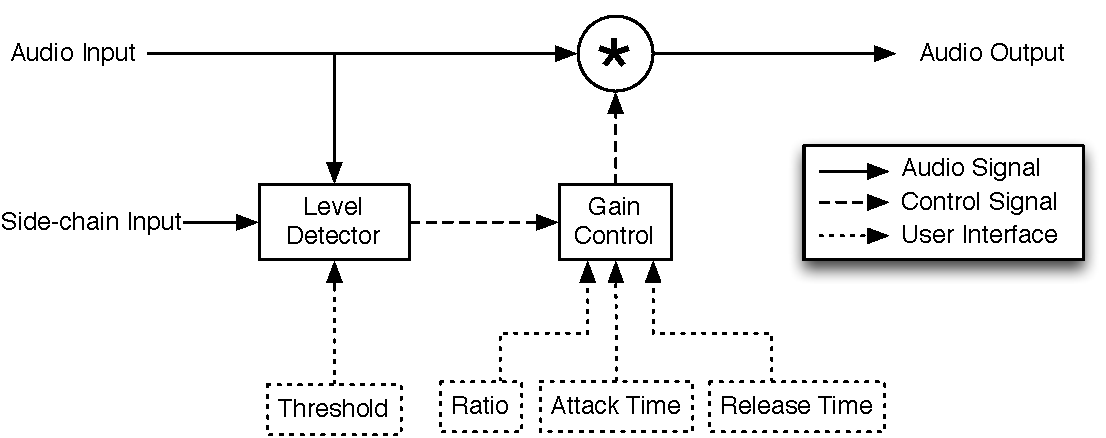
\includegraphics[width=\linewidth]{hypercomp/SimpleCompressor.pdf}
  \caption{Block diagram of a simple traditional dynamic range
    compressor.}
  \label{fig:comp-block}
\end{figure*}

\subsection{Side-Chain Compression}
\label{sec:side-chain-compr}
Compressors often have an additional operational mode that is the
primary inspiration for Hypercompression. We know that compressors
automatically reduce the gain of a signal that exceeds a given
threshold. Some compressors allow us to attenuate the level of a
signal when a \emph{different} signal exceeds the threshold
level. Models that suports side-chain compression have a second audio
input. When we switch the compressor into side-chain mode, the
compressor attenuates the first signal only when the second signal
exceeds the threshold.

Side-chain compression is often used to moderate the balance of kick
drum and bass guitar. If the bass guitar is briefly attenuated just
enough just the right amount each time the kick drum hits, we can set
the kick and bass guitar at exactly the gain levels we want without
one masking the other. Because the bass guitar is only briefly
attenuated, it will not be perceived as any quieter.

In this example we use the kick drum to create a gain envelope for our
bass guitar. The kick \emph{pushes} the bass to make room for
itself. The attack time and release time parameters give control over
this behavior in the temporal domain. The next step is to
expand this model to add control in the spatial domain.

\section{Ambisonics}
\label{sec:ambisonics}
Ambisonics is a technique for encoding and decoding three-dimensional
surround sound audio.\cite[-15mm]{Gerzon1973,Gerzon1985} Ambisonic
audio differs from other surround sound formats like $5.1$ and $7.1$
in that it does not depend on a particular speaker configuration. An
ambisonic recording can be decoded on any surround sound speaker
configuration without disarranging the spatial contents of the audio
recording.

Imagine we use an omnidirectional microphone to record an acoustic
instrument at a sample rate of 44.1 kHz. We sample and record 44100
samples every second that represent the air pressure at the microphone
capsule during the recording. Our omni-directional microphone is
designed to treat sound arriving from all angles equally. The
omnidirectional microphone sums together sounds arriving from all
angles and the acoustic directional information is lost.

If we want to encode, decode, transmit, or play audio that preserves
full sphere 360 degree information, ambisonics offers a solution.
Ambisonic audio uses \textit{spherical harmonics} to encode surround
sound audio that preserves the direction-of-arrival information that
discrete channel recordings (such as mono and stereo) cannot fully
capture.

\subsection{Spherical Harmonics}
\label{sec:spherical-harmonics}
We know that we can construct any monophonic audio waveform by summing
a (possibly infinite) number of harmonic sine waves (Fourier
series).\sidenote{An excellent description of the transformation between
  the time domain and frequency domain can be found at
  \url{http://betterexplained.com/articles/an-interactive-guide-to-the-fourier-transform/}}
For example, by summing odd \textit{order} sine harmonics at a given
frequency $f$, $(1f, 3f, 5f, 7f, \ldots )$, we generate a square wave
with fundamental frequency $f$. As the order increases, so does the
temporal resolution of our square wave.

By summing sinusoidal harmonics, we can generate any continuous
waveform defined in two dimensions (one input parameter and one
output). Similarly, by summing \emph{spherical harmonics}, we can
generate any continuous shape defined over the surface of a
three-dimensional sphere (two input parameters, or polar angles, one
output). Where a traditional monophonic audio encoding might save one
sample 44100 times per second, an ambisonic encoding would save one
sample \emph{for each spherical harmonic} 44100 times per second. This
way we capture a three-dimensional sound image at each audio sample.
The number of spherical harmonics we encode is determined by our
\textit{ambisonic order}. As our ambisonic order increases, so does
the angular resolution of our result on the surface of the sphere.

\subsection{Spherical Harmonic Definition}
For encoding and decoding ambisonics, the convention is to use the
real portion of spherical harmonics as defined in
equation~\ref{eq:spherical}, where:
\begin{itemize}
\item $Y_{n}^{m}(\varphi,\vartheta)$ is a spherical harmonic that
is:\marginnote{Some literature on spherical harmonics swaps the names
  of \textit{order} and \textit{degree}. In this thesis we use
  $Y_{order}^{degree}$. In literature where $Y_{degree}^{order}$ is
  used, the function of the subscript and superscript remain
  unchanged; only the names are inconsistent.}
\begin{itemize}
\item of order, $n$
\item of degree, $m$
\item defined over polar angles $(\varphi, \vartheta)$
\end{itemize}
\item $N_n^{|m|}$ is a normalization factor.\sidenote{In ambisonic
    literature (and software), there are multiple incompatible
    conventions for the normalization of spherical harmonics. The
    Hypercompressor uses the \textit{Furse-Malham} (FuMa)
    normalization convention.}
\item $P_n^{|m|}$ is the associated Legendre function of order $n$
  and degree $m$.
\end{itemize}
\begin{equation}
Y_{n}^{m}(\varphi,\vartheta)=N_n^{|m|}P_n^{|m|}(\sin{\vartheta})
\begin{cases}\label{eq:spherical}
\sin{|m|\varphi},&  \text{for $m<0$}\\  
\cos{|m|\varphi},& \text{for $m\geq 0$}\\
\end{cases}
\end{equation}
Given equation~\ref{eq:spherical}, we can define an ambisonic
audio recording as:
\begin{equation}
f(\varphi,\vartheta,t)=\sum\limits_{n=0}^N\sum\limits_{m=-n}^nY_n^m(\varphi,\vartheta)\phi_{nm}(t)
\label{eq:ambisonics}
\end{equation}
Where:
\begin{itemize}
\item $\varphi$ and $\vartheta$ describe the polar angle of sound
  arrival in two dimensions.\sidenote{Note that ambisonics uses polar
    angles to describe the angle of arrival of sound. These are
    similar to spherical coordinates, minus the inclusion of
    \textit{radial distance}. Distance is not part of the ambisonic
    specification.}
\item $t$ is time
\item $\phi_{nm}(t)$ are our \textit{expansion coefficients}, described
  below.
\end{itemize}
\begin{figure}[h]
  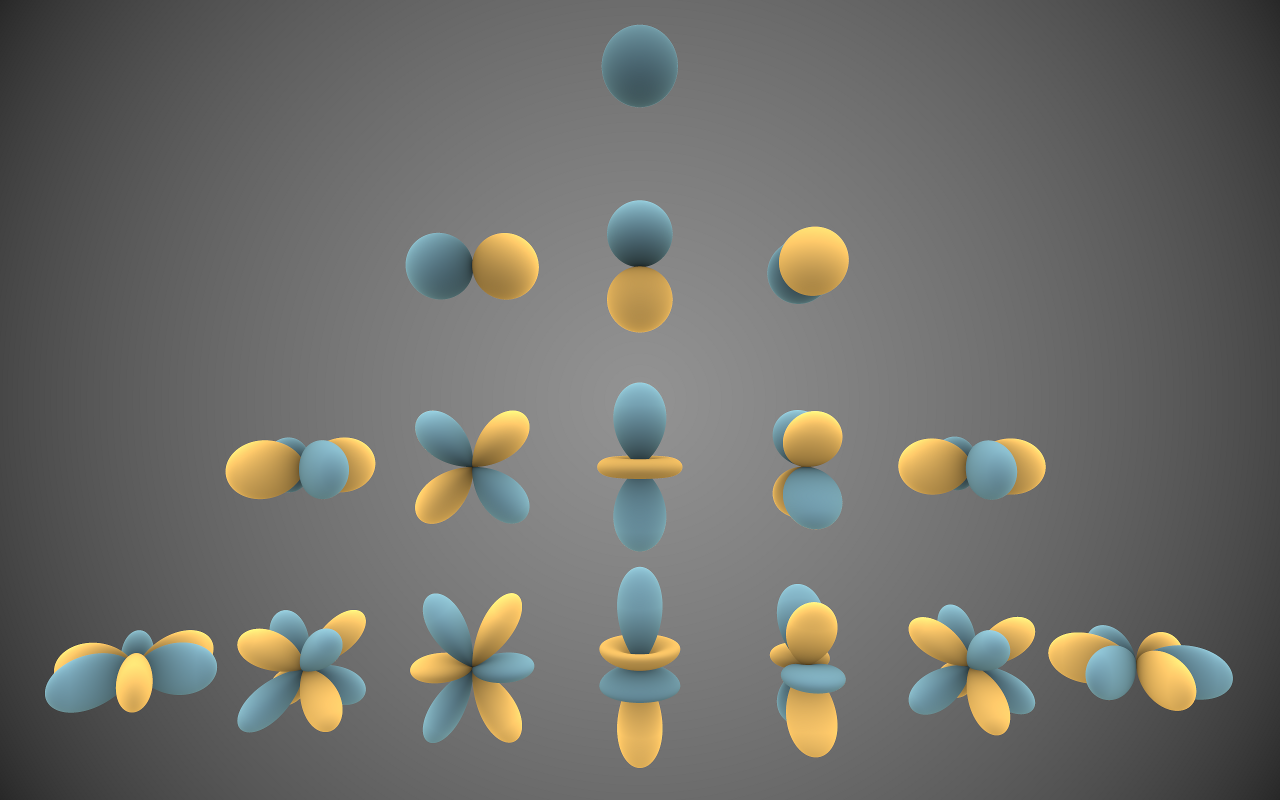
\includegraphics[width=\linewidth]{SphericalHarmonics.png}
  \caption{Spherical harmonics $0$th order (top row) through $3$rd
    order (bottom row). This for image shows the output of
    $Y_{n}^{m}(\varphi,\vartheta)$ for $n=0,n=1,n=2,$and $n=3$. The
    distance of the surface from the origin shows the value at that
    angle. Darker blue regions are positive, while lighter yellow
    regions are negative. Image credit: Ingo Quilez, licensed under
    \textit{Creative Commons Attribution-Share Alike 3.0 Unported}.}
  \label{fig:spherical-harmonics}
\end{figure}

\subsection{Spherical Harmonic Expansion Coefficients}
\label{sec:spher-harm-expans}
In our monophonic recording example, we save just one digital sample
44100 times per second, with each saved value representing the air
pressure at a point in time. We know that by summing the correct
combination of spherical harmonics, we can describe any continuous
function over the surface of a sphere. Instead of sampling air
pressure directly, we sample a coefficient describing the weighting of
each spherical harmonic 44100 times per second. The resulting sphere
encodes the pressure including the direction of arrival
information. The weighting coefficients or \textit{expansion
  coefficients} are recorded in our audio file instead of values
representing air pressure directly. Now, by summing together our
weighted spherical harmonics, we can reconstruct the fluctuations in
pressure including the angle of arrival information. We can recall
this snapshot of information at our 44.1 kHz audio sample rate.

\subsection{Ambisonic Encoding}
\label{sec:usage}
There are two ways to create an ambisonic recording. First, we can use
a soundfield microphone to record an acoustic soundfield. Soundfield
microphones like the one developed by Calrec Audio can capture angle
of arrival information with the spatial resolution of first order
ambisonics.\cite[-1in]{Ferrar1979} Alternatively, we can algorithmically
encode pre-recorded sources, creating virtual sources in an
ambisonic bus.\cite[-0.4in]{Malham1995}

\section{Ambisonic Conventions used for Hypercompression}
\label{sec:ambis-conv-used}
This thesis follows ambisonic convention for describing axis of
rotation. The x-axis points forward, the y-axis point left, and the
z-axis points up. Polar angles are used to describe orientation with
$0\degree$ azimuth being forward, and increasing as we move to the
left. $0\degree$ elevation also points forward, and increases as we
move upward, with $90\degree$ being strait up along the z-axis. When
working with ambisonics, multiple inconpatible conventions exist for
ordering and normalizing spherical harmonics.\cite{Nachbar2011} The
Hypercompressor uses \textit{Furse-Malham} normaliation
(FuMa)\cite{Malham2003}, and first order ambionics with
\textit{B-format}\cite{Hollerweger2008} channel ordering. B-format
ordering labels the four first-order ambisonic channels as W, X, Y,
and Z, with W being the spherical harmonic of order zero and degree zero,
and X, Y, and Z being the ressure gradient components along their
respective axes. 

\section{Hypercompressor Design}
\label{sec:hypercomp-design}
\begin{figure*}
  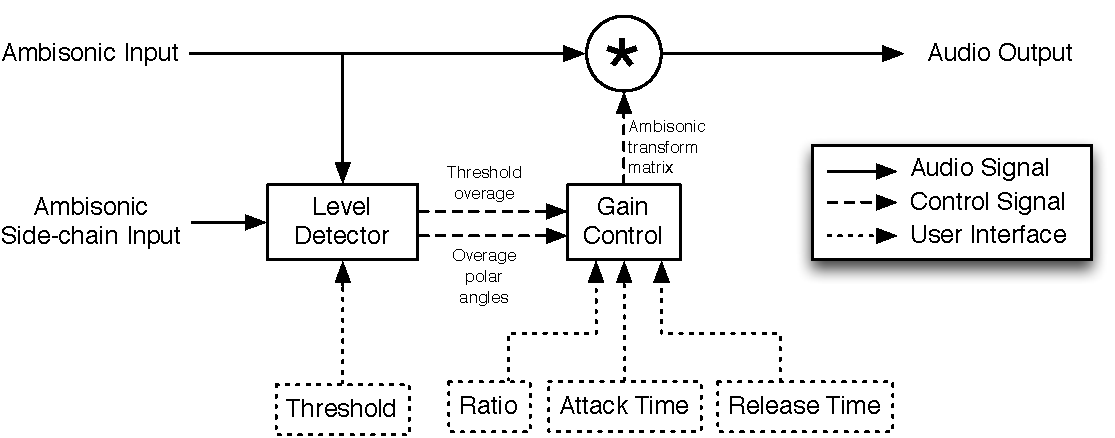
\includegraphics[width=\linewidth]{hypercomp/AmbisonicCompressor.pdf}
  \caption{Block diagram of the Hypercompressor.}
  \label{fig:hypercomp-block}
\end{figure*}
\noindent The Hypercompressor (or ambisonic compressor) combines the traditional
model of compression with the surround sound capability of
ambisonics. Given ambisonic input, and an optional ambisonic
side-chain input, the ambisonic compressor is intended to process our
input material in one of two modes:
\begin{enumerate}
\item Standard mode: We set a compression threshold, similar to on a
  traditional compressor. When a region in our surround sound input
  material exceeds the set threshold, the compressor engages and
  attenuates only that region.
\item Side-chain mode: This mode takes advantage of a second ambisonic
  input to our signal processor. When the gain of spatial region in
  our secondary input exceeds our threshold, we attenuate that same
  region in the the main input, and output the results.
\end{enumerate}
In both modes, our ambisonic compressor must attenuate and release
attenuation according to the attack time and release time
parameters. The block diagram for our new hypercompressor
(figure~\ref{fig:hypercomp-block}) can remain largely unchanged from
the the block diagram for our traditional compressor in
figure~\ref{fig:comp-block}. The most important changes are:
\begin{itemize}
\item Our audio signals must be updated to handle encoded
  ambisonics. This is as simple as increasing the number of channels
  on each solid black connection in figure~\ref{fig:comp-block}. The
  hypercompressor works with first order ambisonics, so every audio
  path must carry four audio channels.
\item On a traditional compressor, the level detector only needs to
  detect the difference between the gain of the input signal and the
  gain specified by the threshold parameter. Our ambisonic level detector
  needs to decode the incoming signals and identify both a threshold
  overage and the region where the overage occurred.
\item Our gain control module needs to listen to the input coming from
  the level detector module and be able to attenuate the specific
  regions that exceed our threshold parameter.
\end{itemize}

\subsection{Level Detection Module}
\label{sec:an-accurate-level}
In \textit{Spatial Transformations for the Alteration of Ambisonic
  Recordings}, Matthias Kronlachner describes
one approach for making a visual ambisonic level meter:\cite{Kronlachner2014} 
\begin{enumerate}
\item Choose a series of discrete points distributed on the surface of
  a sphere. Ideally the points are equally distributed, so the
  vertices of platonic solid shapes like the dodecahedron (12-sided
  polyhedron) and icosahedron (20-sided polyhedron,
  figure~\ref{fig:icosahedron}) work well. For spatial accuracy,
  Kronlachner recommends a spherical $t$-design with 240 points
  described by Hardin and Sloane.\cite{Hardin1996}
\item Evaluate each spherical harmonic at every point chosen. Cache
  the results in a matrix. 
\item With the cached spherical harmonics, it is then possible to
  calculate the RMS and peak values more efficiently at the audio
  rate.
\item A level meter does not need to refresh the display at the audio
  sample rate, so it is acceptable to interpolate between the points
  on the sphere and update the graphical representation at the
  control rate, which could be as slow as 30 Hz (approximately every
  33 milliseconds).
\end{enumerate}
\begin{marginfigure}
  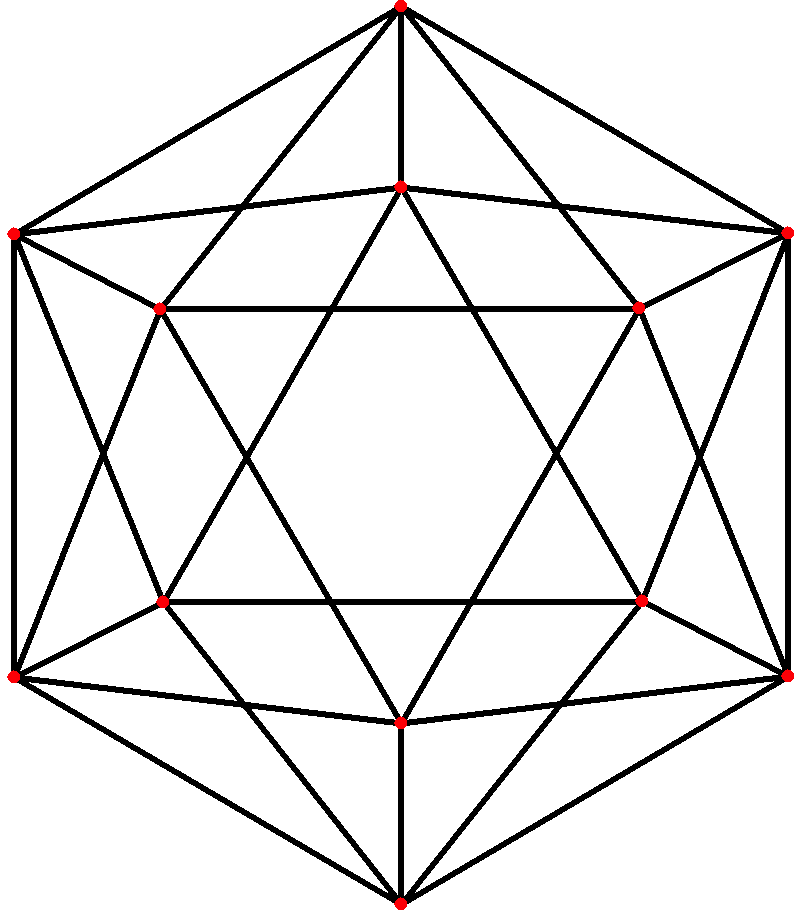
\includegraphics{hypercomp/Icosahedron.png}
  \caption{An icosahedron.}
  \label{fig:icosahedron}
\end{marginfigure}
A similar approach can be used to make an ambisonic level
detector. However, a compressor needs to react much quicker than a
level meter. The compressor cannot even \emph{begin} to engage until
the level meter has responded, and attack times faster than 33
milliseconds are common in conventional compression. Every point on
the sphere requires a buffer to calculate the RMS. We also need to
decode ambisonics at the audio sample rate and keep track of peak
values. Ideally we would also interpolate between the points.

\subsection{An Efficient Level Detection Module}
\label{sec:hyperc-level-detect}
The Hypercompressor needs to detect the level of our ambisonic input
material and identify (as quickly as possible) when and where the
signal exceeds the compressor threshold. In the interest of
computational efficiency, the first level detector I wrote attempted
to extract overage information with minimal ambisonic decoding and
signal processing.
\begin{enumerate}
\item To accurately play a first order ambisonic encoding, we need a
  minimum of 6 speakers placed around the listener. In this level
  detector, we calculate the root mean square (RMS) average at the
  center of 6 lobes corresponding to the first order spherical
  harmonics: front, rear, left, right, top, and bottom.
\item Calculate a map of the influence of each lobe on the surround
  image\TODO{Clean}
  (figures~\ref{fig:hypercomp-mathematica},~\ref{fig:hypercomp-inf-maps}). For
  example, pan a monophonic sound directly forward in an ambisonic
  mix, cache an image of the resulting sound sphere. Save one image
  for each of the 6 lobes.
\item We have 6 images, each representing one of the 6 lobes of our
  first order ambisonic spherical harmonics. In step 1, we calculated
  the RMS level at each of the corresponding points on our surround
  sphere. Use the 6 RMS levels to weight each of our 6 maps. The sum
  of the weighted maps shows the gain distributed across our ambisonic
  sphere.
\end{enumerate}

\begin{figure}[]
  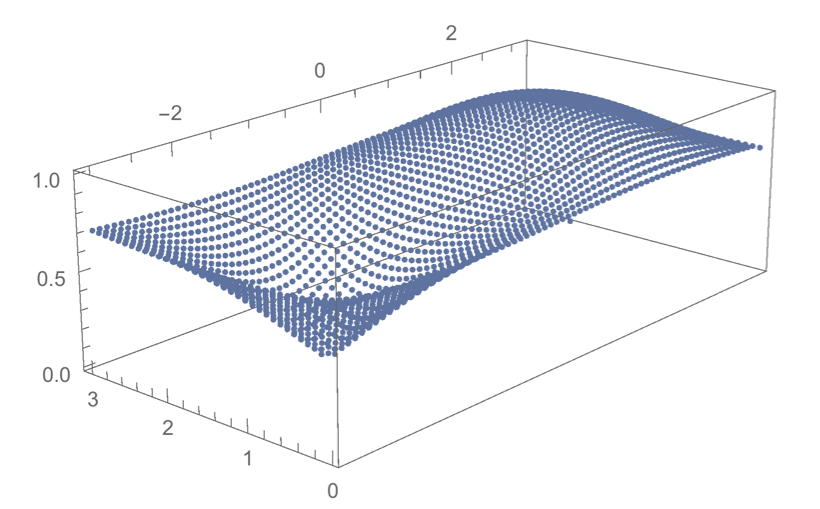
\includegraphics[width=\linewidth]{hypercomp/AmbisonicFieldAngle.png}
  \caption{Calculating the cylindrical projection of single ambisonic panned
    source in the Wolfram Mathematica software package}
  \label{fig:hypercomp-mathematica}
\end{figure}

\begin{figure}[]
 
\includegraphics[width=3.5cm]{hypercomp/left_x72.png}
 
\includegraphics[width=3.5cm]{hypercomp/above_x72.png}
 
\includegraphics[width=3.5cm]{hypercomp/front_x72.png}
 % 
\includegraphics[width=3.5cm]{hypercomp/right_x72.png}
 % 
\includegraphics[width=3.5cm]{hypercomp/below_x72.png}
 % 
\includegraphics[width=3.5cm]{hypercomp/rear_x72.png}
  \caption{Influence maps of 3 first-order spherical harmonics: left, top, and
    front. Pure white is $-0$~dBFS black is -inf~dBFS. Cylindrical projection.}
  \label{fig:hypercomp-inf-maps}
\end{figure}

\paragraph{Results:}If the input to the level detector is encoded as
an ambisonic plane wave, this level detector does yield accurate
results.  In the more common case, when our ambisonic input material
contains multiple sources that are each ambisonically panned to
different positions, this interpolation technique does not accurately
calculate the RMS at any angle. In simple cases, where we can be sure
our input material is appropriate, the technique described here might
be useful, but in most cases, a different approach will be more
effective.

\begin{figure}[h]
%  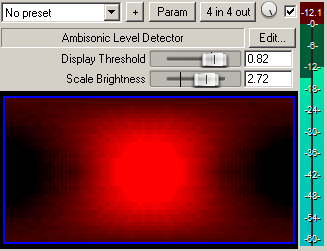
\includegraphics{hypercomp/LevelDetect_front.png}
  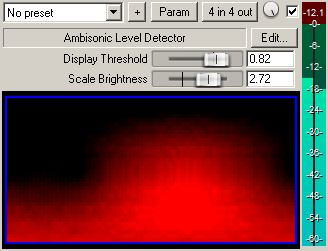
\includegraphics{hypercomp/LevelDetect_45_down.png}
  \caption{The Hypercompressor visualizer written for the efficient
    ambisonic level detector. The surround sphere is projected to a
    cylinder and unwrapped on the flat surface. In this image, a
    monophonic source is panned slightly down and to the right
    ($-45\degree$ azimuth, $-45\degree$ elevation).}
  \label{fig:hypercomp-inf-map-angle}
\end{figure}

\subsection{Ambisonic Gain Control Module}
\label{sec:ambis-gain-contr}
The spherical harmonics defined in equation~\ref{eq:ambisonics} form a
set of orthogonal basis functions. If we define a sequence for our
spherical harmonics and spherical harmonic expansion coefficients, we
can treat the expansion coefficients as vectors and perform matrix
operations on them that rotate, warp, and re-orient our
three-dimensional surround sound image.\cite{Pomberger2011} The
ability to mathematically warp and manipulate our surround sound image
makes ambisonics the perfect choice for implementing a surround sound
compressor.

\paragraph{The Focus Transform} One transform that lets us attenuate a
region of the surround sound sphere is the \textit{focus} transform
distributed as part of the open source Ambisonic Toolkit
(ATK)\sidenote{\url{http://www.ambisonictoolkit.net/}} This transform
is intended to focus on transform is intended to focus on the 
\cite{Anderson2009}
\begin{fullwidth}
\[ \left( \begin{array}{cccc}
\frac{1}{1 + \sin|w|} & 
\frac{1}{\sqrt{2}} \frac{\sin(w)}{1 + \sin|w|}  & 
0 &
0 \\
\sqrt{2}\frac{sin(w)}{1 + \sin|w|} & % LG1
\frac{1}{1 + \sin|w|} &                    % LG0
0 & 
0 \\
0 & 
0 &
\frac{\cos(w)}{1 + \sin(w)} &
0 \\
0 &
0 &
0 &
\frac{\cos(w)}{1 + \sin|w|} 
\end{array} \right)
\]
\end{fullwidth}
%%% Local Variables:
%%% mode: latex
%%% TeX-master: "CharlesHolbrow_MAS_Thesis"
%%% End:


\backmatter

\chapter*{Acknowledgements}
\label{ch:acknowledgements}

\begin{fullwidth}
Thanks to Tod Machover, for your continuous support and encouragement,
for sharing your process, and for help and support integrating \thesis
into \textit{Of Experience}.

Thanks to James Andy Moorer and Joe Paradiso for support, guidance and
mentorship.\TODO{verify spelling}

Thanks to professor Alex Case for the most inspiring my love for
music, audio engineering, and illuminating the magical subtleties of
dynamic range compression.

Thanks to Wonshik Choi and Niyom Lue for your infinite patience,
guidance, and for welcoming me to MIT in 2008. Only you could have
taught a music major to enjoy linux, DSP, and spectroscopy.

Thanks to Shawn Drost for directly and indirectly giving me confidence
as a software developer.

Thanks to my UMass Lowell Piano teachers for taking chance with me,
and putting up with me for four years. Anthony Mele, Elizabeth
Skavish, Bonnie Anderson, and Thomas Stumpf - You believed in me
before I did. I'm probably the only student ever who was lucky enough
to study with all four of you. :P

Thanks to Gene Atwood for being considerate of everyone, and showing
me how important that is -- And for screaming in to a microphone when
I needed some screams.

Thanks to Ben Bloomberg for being my peer and my mentor at the same
time. Thanks for bringing me into the Opera group in 2008 and bringing
me back in 2014. Thanks to Bryn Bliska, for proposing polytempic
modulation, and sharing letting me work out the maths. Thanks to
Rebecca Kleinberger and Akito Van Troyer for your unending support and
encouragement. 

Thanks to Helen Corless for being amazing supportive even when I am in
the absolute pits of grad student existence. Thank you for always
reminding me what music is really about, and for challenging me like
no one else can.

Thanks to my grandparents for leading by example, and teaching
kindness and dedication, and for endless support in education.

Thanks to Hilary, Giles, and Felicity for always inspiring me with
kindness, honesty, and wisdom. 

And thanks to my parents, Gwen and Mark for forcing me to get an
education before I was wise enough to know I wanted one. Thank you for
all your love and support in everything ever I have ever done.
\end{fullwidth}
%%% Local Variables:
%%% mode: latex
%%% TeX-master: t
%%% End:


\bibliography{library}
\bibliographystyle{plainnat}

\end{document}


%%% Local Variables:
%%% mode: latex
%%% TeX-master: t
%%% End:
